\documentclass{article}

\title{\sc\LARGE CSCA67 Tutorial, Week 7\\
{\Large Oct. 26th-Oct. 30th, 2015}}
\date{}
\author{\sc Compiled by {\em G. Singh Cadieux}\\[1ex]
\sc Adapted from\\
A. Bretscher, \href{http://www.utsc.utoronto.ca/~bretscher/a67/lectures/implication.pdf}{\em Implication and Direct Proofs worksheet},\\
A. Bretscher, {\em Introduction to Proofs Lecture Notes} \&\\
A. Bretscher, {\em CSCA65 Lecture Notes: Formal Languages - Logic}}

\usepackage{fullpage}
\usepackage{amsmath,amssymb}
\usepackage{color}
\usepackage{multirow}
\usepackage{tikz}
\usepackage{hyperref}
\usepackage{array}

\setlength{\parindent}{0pt}

\begin{document}
\maketitle

\section{\sc Formal Logic}

A \textsc{statement} (also known as a \textsc{proposition}) is a sentence that can be evaluated to be true or false.

\subsection*{Q: {\em Which of the following are statements?}}
\begin{tabular}{p{0.5\textwidth}|p{0.5\textwidth}}
(1) $2\times 4=8$&statement (true)\\\noalign{\smallskip}
(2) $5=9$&statement (false)\\\noalign{\smallskip}
(3) It will snow this afternoon.& statement (value is unknown, but must evaluate to true or false)
\\\noalign{\smallskip}
(4) If I am happy, then I am not happy.& statement (false)\\\noalign{\smallskip}
(5) Give the definition of a statement.& not a statement\\\noalign{\smallskip}
(6) This statement is false.& not a statement (cannot be either true or false - if it is true, then it is false; if it is false, then it is true)\\\noalign{\smallskip}
(7) This statement is true.& not a statement (value cannot be determined, could be evaluated as either true or false)
\end{tabular}\\[1em]
We represent statements using symbols (which are often arabic or Greek letters).\\
For example, we can let $p$ represent the statement ``It is raining," and $q$ represent the statement ``I have an umbrella."\\[1em]
We can build more complex statements (known as ``compound statements") by combining statements using any of the following \textsc{connectives}, or \textsc{operators}.\\[1ex]
\begin{tabular}{ccclc}
Symbol&Meaning&\multicolumn{2}{l}{Example}&\multirow{6}{*}{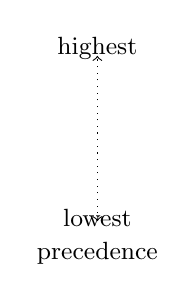
\begin{tikzpicture}
\draw[<->,dotted] (0.1,0) -- (0.1,2.1);
\node at (0.1,2.2) {\small highest};
\node[align=center] at (0.1,-0.2) {\small lowest\\\small precedence};
\end{tikzpicture}}
\\\cline{1-4}\noalign{\addvspace{1pt}}\cline{1-4}
$\neg$&``not"&$\neg p$& It is \textit{not} raining.&\\
$\wedge$&``and"&$p\wedge q$& It is raining \textit{and} I have an umbrella.&\\
$\vee$&``or"&$p\vee q$& It is raining \textit{or} I have an umbrella.&\\
$\to$&``implies"&$p\to q$& \textit{If} it is raining, \textit{then} I have an umbrella.&\\
$\leftrightarrow$&``if and only if"&$p\leftrightarrow q$& It is raining \textit{if and only if} I have an umbrella.
\end{tabular}\\[2em]
We may also use parentheses to group statements and connectives. When parentheses are omitted, the connectives are applied according to the precedence rules (also called the ``order of operations").\\[1ex]
For example, when $\neg A\wedge B$ is parenthesized, it becomes $\neg(A)\wedge B$, since $\neg$ has higher precedence than $\wedge$. Note that this is entirely different from $\neg(A\wedge B)$.\\
Likewise, when $A\wedge B\to\neg C\vee D\wedge E$ is parenthesized, according to the precedence rules, it becomes $(A\wedge B)\to((\neg C)\vee (D\wedge E))$.\\[1ex]
When an operator is repeated, sub-expressions are usually grouped to the right. For example, when $A\to B\to C$ is parenthesized, it becomes $A\to(B\to C)$.

\subsection*{{\normalsize Given the statements\\
$p:$ ``You are in Seoul."\\
$q:$ ``You are in Kwangju."\\
$r:$ ``You are in South Korea."}\\[1ex]
Q: {\em Translate the following statement into formal logic:\\
``If you are not in South Korea, then you are not in Seoul or Kwangju."}}
We start with the most general statement: from the language ``if\ldots then\ldots", we know that the statement is an implication, with ``you are not in South Korea" as the antecedent (first half) and ``you are not in Seoul or Kwangju" as the consequent (second half).\\[1ex]
``You are not in South Korea" is the negation of $r$, and ``you are not in Seoul or Kwangju" is the negation of ``you are in Seoul or you are in Kwangju".\\[1ex]
``You are in Seoul or you are in Kwangju" is the disjunction (``or") of $p$ and $q$.\\[1ex]
Thus, in formal logic, our statement is $r\to\neg(p\vee q)$.\\[1ex]
Alternatively, because of the ambiguity of the English language, we may consider ``you are not in Seoul or Kwangju" to be the conjunction (``and") of ``you are not in Seoul" and ``you are not in Kwangju", which are, respectively, the negation of $p$ and $q$. Then our statement would be $r\to\neg p\wedge\neg q$.

\subsection*{Q: {\em Translate the following formal statement into everyday English:
$q\to(r\wedge\neg p)$}}
Here, we start with the most specific statement: $\neg p$ is the negation of ``you are in Seoul", which we express in English as ``you are not in Seoul".\\[1ex]
Then, $r\wedge\neg p$ is the conjunction (``and") of ``you are not in Seoul" and ``you are in South Korea", which we express as ``you are in South Korea and you are not in Seoul".\\[1ex]
Finally, we translate the implication to ``if\ldots then\ldots", with ``you are in Kwangju" as the antecedent (first half) and ``you are in South Korea and you are not in Seoul" as the consequent (second half).\\[1ex]
Thus, in English, our statement is ``If you are in Kwangju, then you are in South Korea and you are not in Seoul".\\[1ex]
Because of the ambiguity of the English language, there are several equivalent ways to structure this sentence. For example, we might say ``If you are in Kwangju, then you are in South Korea \textit{but} you are not in Seoul", or simply ``If you are in Kwangju, then you are in South Korea but not in Seoul".

\subsection{\sc Truth Tables}
A \textsc{truth table} is a table showing all possible truth values for a statement, depending upon the statements that make it up.\\[1ex]
When we construct a truth table for a statement $A$ containing operator(s) and constituent statements $A_1,\,A_2,\,\ldots$, we show the possible truth values of $A_1,\,A_2,\,\ldots$ on the left side of the table, and the corresponding truth values for $A$ on the right side of the table.\\
Each row of the truth table represents the truth value $A$ given the truth values of $A_1,\,A_2,\,\ldots$ in that row. \\[1ex]
The most basic truth table is the truth table for the single statement $p$, shown below. $p$ can take either a true (T) or false (F) value.\\[1ex]
\textsc{Note} that the order of the rows in a truth table is not significant, although a conventional ordering can make the truth table easier to read.
\begin{figure}[h]
\begin{minipage}{0.06\textwidth}\centering{\begin{tabular}{c}
$p$\\\hline
T\\
F
\end{tabular}}\end{minipage}
\begin{minipage}{0.12\textwidth}\centering{\begin{tabular}{c|c}
$p$&$\neg p$\\\hline
T&F\\
F&T
\end{tabular}}\end{minipage}
\begin{minipage}{0.18\textwidth}\centering{\begin{tabular}{cc|c}
$p$&$q$&$p\wedge q$\\\hline
T&T&T\\
T&F&F\\
F&T&F\\
F&F&F
\end{tabular}}\end{minipage}
\begin{minipage}{0.18\textwidth}\centering{\begin{tabular}{cc|c}
$p$&$q$&$p\vee q$\\\hline
T&T&T\\
T&F&T\\
F&T&T\\
F&F&F
\end{tabular}}\end{minipage}
\begin{minipage}{0.18\textwidth}\centering{\begin{tabular}{cc|c}
$p$&$q$&$p\to q$\\\hline
T&T&T\\
T&F&F\\
F&T&T\\
F&F&T
\end{tabular}}\end{minipage}
\begin{minipage}{0.18\textwidth}\centering{\begin{tabular}{cc|c}
$p$&$q$&$p\leftrightarrow q$\\\hline
T&T&T\\
T&F&F\\
F&T&F\\
F&F&T
\end{tabular}}\end{minipage}
\end{figure}\\
\textsc{A truth table} is particularly useful for assessing the possible truth values of a complex statement (i.e., one which contains many operators and/or constituent statements). When constructing such a truth table, we break the statement into smaller clauses and assess the truth value of each, before combining them into the original statement.\\
For example, here is a (partial) truth table for $(\neg r\vee q)\wedge p$:
\begin{center}
\begin{tabular}{ccc|c|c|c}
$r$&$q$&$p$&$\neg r$&$\neg r\vee q$&$(\neg r\vee q)\wedge p$\\\hline
T&T&T&F&T&T\\
T&T&F&F&T&F\\
T&F&T&F&F&F\\
\multicolumn{3}{c|}{\vdots}&\vdots&\vdots&\vdots
\end{tabular}
\end{center}

\subsection*{{\normalsize Given the statements\\
$p$: ``Andy is hungry."\\
$q$: ``The refrigerator is empty."\\
$r$: ``Andy is mad."}\\[1ex]
Q: {\em Construct a truth table for the following statement:\\
``If Andy is hungry and the refrigerator is empty, then Andy is mad."}}

First, we must translate this statement into formal logic. From the language ``if\ldots then\ldots", we know that the statement is an implication, with ``Andy is hungry and the refrigerator is empty" as the antecedent and ``Andy is mad" as the consequent. ``Andy is hungry and the refrigerator is empty" is the conjunction of $p$ and $q$.\\
Thus, in formal logic, our statement is $p\wedge q\to r$.\\[1ex]
To build our truth table, we begin with the smallest constituent statements, $p$, $q$, and $r$, and detemine all possible combinations of truth values for these.\\[1ex]
Then, we identify the next smallest sub-statement, based on precedence rules and parentheses - in this case, it is $p\wedge q$. We determine the truth values of this statement using the truth values of the statements that make it up - in this case, $p$ and $q$.\\[1ex]
We continue doing this until we have truth values for all sub-statements within our original statement. Finally, we use these truth values to determine the truth values of the original statement.
\begin{center}
\begin{tabular}{cccc>{\color{red}}c>{\color{red}}cc|cccc>{\color{red}}c|>{\color{red}}c|c}
$p$&$q$&$r$&\multirow{6}{*}{$\Rightarrow$}&
$p$&$q$&$r$&$p\wedge q$&\multirow{6}{*}{$\Rightarrow$}&
$p$&$q$&$r$&$p\wedge q$&$p\wedge q\to r$\\
\cline{1-3}\cline{5-8}\cline{10-14}T&T&T&&T&T&T&T&&T&T&T&T&T\\
T&T&F&&T&T&F&T&&T&T&F&T&F\\
T&F&T&&T&F&T&F&&T&F&T&F&T\\
T&F&F&&T&F&F&F&&T&F&F&F&T\\
F&T&T&&F&T&T&F&&F&T&T&F&T\\
F&T&F&&F&T&F&F&&F&T&F&F&T\\
F&F&T&&F&F&T&F&&F&F&T&F&T\\
F&F&F&&F&F&F&F&&F&F&F&F&T
\end{tabular}
\end{center}

\subsection*{{\normalsize Suppose that this statement is true, and that Andy is not mad and the refrigerator is empty.}\\
Q: {\em Is Andy hungry?}}
Each of our assumptions assigns a truth value to a statement in our truth table:
\begin{itemize}
\item ``this statement is true" $\Rightarrow$ $p\wedge q\to r$ is true
\item ``Andy is not mad" $\Rightarrow$ $r$ is false
\item ``the refrigerator is empty" $\Rightarrow$ $q$ is true
\end{itemize}
We are then being asked to find the truth value of $p$, ``Andy is hungry".\\[1ex]
We find the row of our truth table which corresponds to the truth values we know.
\begin{center}
\begin{tabular}{ccc|c|c}
$p$&$q$&$r$&\ldots&$p\wedge q\to r$\\\hline
T&T&T&\multirow{8}{*}{\ldots}&T\\
T&T&F&&F\\
T&F&T&&T\\
T&F&F&&T\\
F&T&T&&T\\
\color{red}F&\color{red}T&\color{red}F&&\color{red}T\\
F&F&T&&T\\
F&F&F&&T
\end{tabular}
\end{center}
We can see that $p$ is false in this row. Thus, Andy is \textit{not} hungry.

\subsection{\sc Logical Equivalence}
Two statements are \textsc{logically equivalent} if they have the same truth table - that is, given the same combination of truth values for their constituent statements, they both have the same truth value.\\[1ex]
For example, using truth tables, we can demonstrate that $p$ and $\neg\neg p$ are logically equivalent:
\begin{center}
\begin{tabular}{ccc|c|c}
$p$&&$p$&$\neg p$&$\neg\neg p$\\
\cline{1-1}\cline{3-5} \color{red}T&&T&F&\color{red}T\\
\color{red}F&&F&T&\color{red}F
\end{tabular}
\end{center}
Likewise, we can demonstrate that $\neg y\wedge (y\vee x)$ and $\neg y\wedge x$ are logically equivalent:
\begin{center}
\begin{tabular}{cc|c|c|c||c}
$x$&$y$&$\neg y$&$y\vee x$&$\neg y\wedge (y\vee x)$&$\neg y\wedge x$\\\hline
T&T&F&T&\color{red}F&\color{red}F\\
T&F&T&T&\color{red}T&\color{red}T\\
F&T&F&T&\color{red}F&\color{red}F\\
F&F&T&F&\color{red}F&\color{red}F\\
\end{tabular}
\end{center}

\subsection*{Q: {\em Show that $\neg(p\wedge q)$ is logically equivalent to $\neg p\vee\neg q$ using truth tables.}}
\begin{center}
\begin{tabular}{cc|c|c||c|c|c}
$p$&$q$&$p\wedge q$&$\neg(p\wedge q)$&$\neg p$&$\neg q$&$\neg p\wedge\neg q$\\\hline
T&T&T&F&F&F&F\\
T&F&F&T&F&T&T\\
F&T&F&T&T&F&T\\
F&F&F&T&T&T&T
\end{tabular}
\end{center}
$\neg(p\wedge q)$ and $\neg p\vee\neg q$ have the same truth table - thus, they are logically equivalent statements.

\subsection{\sc Using Venn Diagrams}
We can consider any statement $a$ to be the statement ``$x\in A$", where $A$ is a set and $x$ is an element.\\[1ex]
Then, if we draw a Venn diagram containing $A$, $a$ is true at every location in the diagram where an element $x$ at that location is in $A$. $a$ is false everywhere else.
\begin{center}
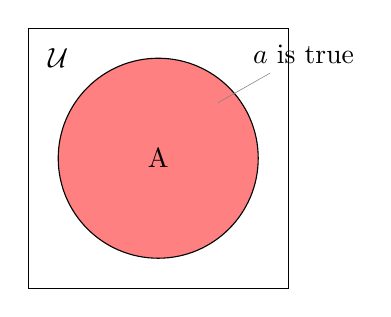
\begin{tikzpicture}
\draw[fill=red!50] (0,0) circle[radius=0.5in];
\draw (-.65in,-.65in) rectangle (.65in,.65in);
\node at (0,0) {A};
\node at (-.5in,.5in) {$\mathcal{U}$};
\node[pin={above right:$a$ is true}] at (.25in,.25in) {};
\end{tikzpicture}
\end{center}

\subsection*{Q: {\em Shade the region(s) where each of the following is true: $\neg a,\;\neg a\vee a,\;\neg a\wedge a$.}}
\begin{center}
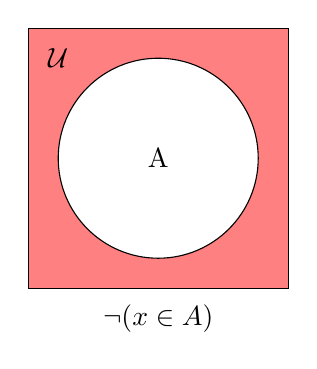
\begin{tikzpicture}
\draw[fill=red!50] (-.65in,-.65in) rectangle (.65in,.65in);
\draw[fill=white] (0,0) circle[radius=0.5in];
\node at (0,0) {A};
\node at (-.5in,.5in) {$\mathcal{U}$};
\node at (0,-.8in) {$\neg(x\in A)$};
\end{tikzpicture}\qquad
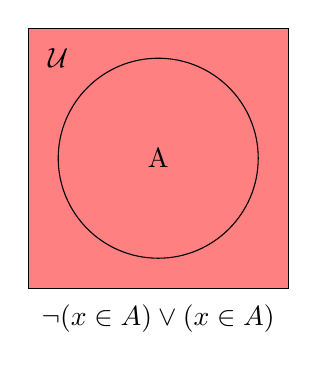
\begin{tikzpicture}
\draw[fill=red!50] (-.65in,-.65in) rectangle (.65in,.65in);
\draw(0,0) circle[radius=0.5in];
\node at (0,0) {A};
\node at (-.5in,.5in) {$\mathcal{U}$};
\node at (0,-.8in) {$\neg(x\in A)\vee(x\in A)$};
\end{tikzpicture}\qquad
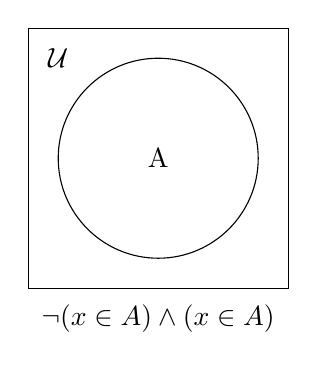
\begin{tikzpicture}
\draw (0,0) circle[radius=0.5in];
\draw (-.65in,-.65in) rectangle (.65in,.65in);
\node at (0,0) {A};
\node at (-.5in,.5in) {$\mathcal{U}$};
\node at (0,-.8in) {$\neg(x\in A)\wedge(x\in A)$};
\end{tikzpicture}
\end{center}
\textsc{Notice} that $\neg a\vee a$ is true for every region in the diagram. This is because, regardless of the truth value of $a$ (or of its constituent statements), $\neg a\vee a$ is always true. This type of statement is known as a \textit{tautology}.\\[1ex]
Notice also that $\neg a\wedge a$ is false for every region in the diagram. This is because, regardless of the truth value of $a$ (or of its constituent statements), $\neg a\wedge a$ is always false. This type of statement is known as a \textit{contradiction}.\\[1em]
We follow the same process to represent a statement with multiple constituent statements.\\
For example, to create a Venn diagram representing $a\wedge b$, we let $a$ be the statement ``$x\in A$" and $b$ be the statement ``$x\in B$", where $A$ and $B$ are sets and $x$ is an element. Then
\begin{center}
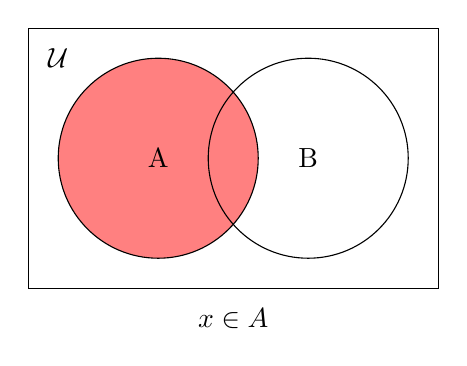
\begin{tikzpicture}
\draw[fill=red!50] (0,0) circle[radius=0.5in];
\draw (0.75in,0) circle[radius=0.5in];
\draw (-.65in,-.65in) rectangle (1.4in,.65in);
\node at (0,0) {A};
\node at (0.75in,0) {B};
\node at (-.5in,.5in) {$\mathcal{U}$};
\node at (0.375in,-.8in) {$x\in A$};
\end{tikzpicture}\quad
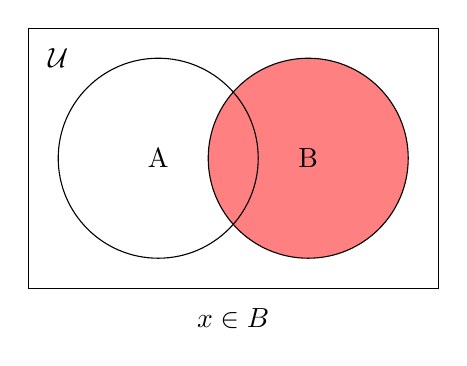
\begin{tikzpicture}
\draw[fill=red!50] (0.75in,0) circle[radius=0.5in];
\draw (0,0) circle[radius=0.5in];
\draw (-.65in,-.65in) rectangle (1.4in,.65in);
\node at (0,0) {A};
\node at (0.75in,0) {B};
\node at (-.5in,.5in) {$\mathcal{U}$};
\node at (0.375in,-.8in) {$x\in B$};
\end{tikzpicture}\quad
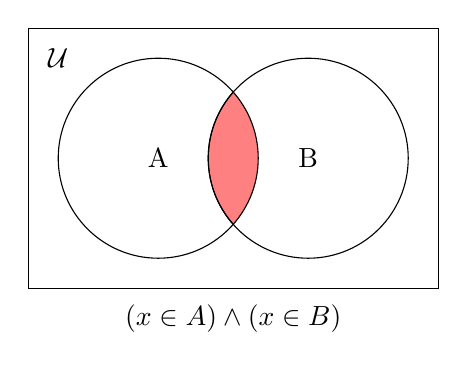
\begin{tikzpicture}
\draw (-.65in,-.65in) rectangle (1.4in,.65in);
\node at (-.5in,.5in) {$\mathcal{U}$};
\begin{scope}
\path[clip] (0,0) circle[radius=0.5in];
\draw[fill=red!50] (0.75in,0) circle[radius=0.5in];
\end{scope}
\draw (0,0) circle[radius=0.5in];
\draw (0.75in,0) circle[radius=0.5in];
\node at (0,0) {A};
\node at (0.75in,0) {B};
\node at (0.375in,-.8in) {$(x\in A)\wedge (x\in B)$};
\end{tikzpicture}
\end{center}

\subsection*{Q: {\em Shade the region(s) where $a\to b$ is false.}}
\begin{center}
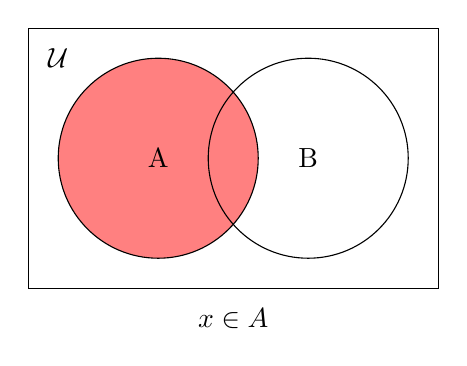
\begin{tikzpicture}
\draw[fill=red!50] (0,0) circle[radius=0.5in];
\draw (0.75in,0) circle[radius=0.5in];
\draw (-.65in,-.65in) rectangle (1.4in,.65in);
\node at (0,0) {A};
\node at (0.75in,0) {B};
\node at (-.5in,.5in) {$\mathcal{U}$};
\node at (0.375in,-.8in) {$x\in A$};
\end{tikzpicture}\quad
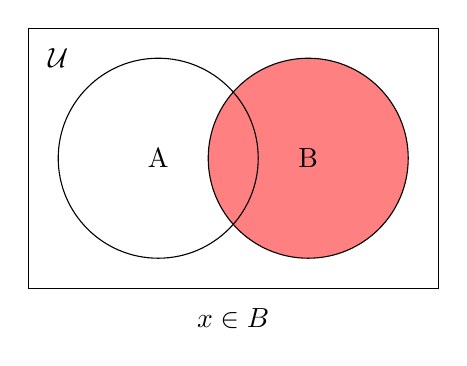
\begin{tikzpicture}
\draw[fill=red!50] (0.75in,0) circle[radius=0.5in];
\draw (0,0) circle[radius=0.5in];
\draw (-.65in,-.65in) rectangle (1.4in,.65in);
\node at (0,0) {A};
\node at (0.75in,0) {B};
\node at (-.5in,.5in) {$\mathcal{U}$};
\node at (0.375in,-.8in) {$x\in B$};
\end{tikzpicture}\quad
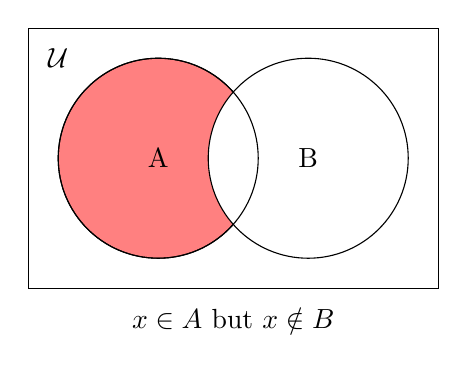
\begin{tikzpicture}
\draw[fill=red!50] (0,0) circle[radius=0.5in];
\draw[fill=white] (0.75in,0) circle[radius=0.5in];
\draw (0,0) circle[radius=0.5in];
\draw (-.65in,-.65in) rectangle (1.4in,.65in);
\node at (0,0) {A};
\node at (0.75in,0) {B};
\node at (-.5in,.5in) {$\mathcal{U}$};
\node at (0.375in,-.8in) {$x\in A$ but $x\notin B$};
\end{tikzpicture}
\end{center}
\textsc{Notice} that this region is the region in which $a$ is true but $b$ is false. Everywhere else (that is, for every other combination of truth values for $a$ and $b$), the implication is true.

\section{\sc Additional practice problems}
{\bf Q: Which of the following are valid propositions?}
\begin{itemize}
\item $2+2=4$
\item $2+3=7$
\item If it is sunny tomorrow, I will go to the beach.
\item What is going on?
\item Stop at the red light.
\end{itemize}
{\bf Q: Which of the following propositions are true?}
\begin{itemize}
\item If $a,b,c$ are two sides and the hypotenuse of a triangle, then $a^2+b^2=c^2$.
\item If $2+2=4$ then pigs can fly.
\item If pigs can fly then pigs can get sunburned.
\item If $2+2=5$ then $2+2=4$.
\end{itemize}
{\bf Q: Use truth tables to prove the following \textit{distributive} properties:}\\[1ex]
$p\wedge(q\vee r)$ is logically equivalent to $(p\wedge q)\vee(p\wedge r)$.\\[1ex]
$p\vee(q\wedge r)$ is logically equivalent to $(p\vee q)\wedge(p\vee r)$.\\[1em]\pagebreak\\
{\bf Q: Use truth tables to prove the following \textit{associative} properties:}\\[1ex]
$p\vee(q\vee r)$ is logically equivalent to $(p\vee q)\vee r$.\\[1ex]
$p\wedge(q\wedge r)$ is logically equivalent to $(p\wedge q)\wedge r$.\\[1em]
There are 3 boxes A, B, C. Exactly one contains gold.\\
Each box has a message on top, but only one of the messages is true.\\
Box A: \textit{Gold is not in this box.}\qquad Box B: \textit{Gold is not in this box.}\qquad Box C: \textit{Gold is in box A.}\\
{\bf Q: Use implication to determine which box the gold is in.}\\[1ex]
\underline{Hint}: Start with \{$p$: Gold is in box A, $q$: Gold is in box B, $r$: Gold is in box C\}, 
and rewrite the messages using these propositions.\\[1em]
{\bf Q: Construct a truth table for the following compound statement:\\
$\neg(\neg(X\vee \neg Y\vee\neg Z) \vee (\neg X\wedge Y\wedge\neg Z))\vee (\neg X\vee (\neg Y\wedge Z))$\\[1em]
{\bf Q: Use a truth table to prove that the statement $((p\vee q)\wedge(\neg p))\to q$ is always true, no matter what $p$ and $q$ are.}

\end{document}